\begin{figure}[H]
    \centering
    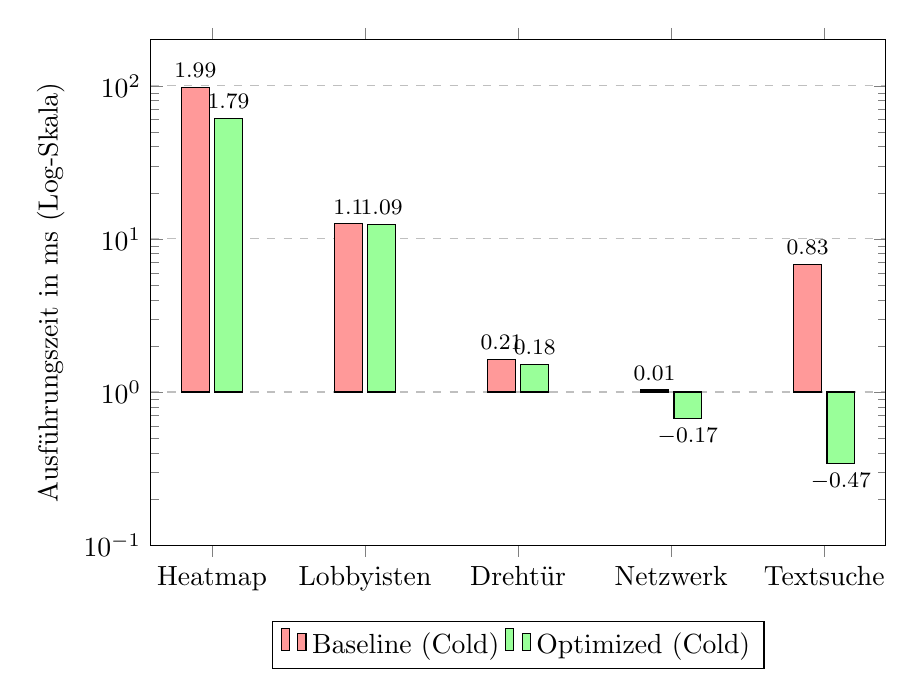
\begin{tikzpicture}
        \begin{axis}[
            ybar,
            width=0.9\textwidth,
            height=8cm,
            symbolic x coords={Heatmap, Lobbyisten, Drehtür, Netzwerk, Textsuche},
            xtick=data,
            ylabel={Ausführungszeit in ms (Log-Skala)},
            ymode=log,
            log basis y={10},
            ymin=0.1, ymax=200,
            nodes near coords,
            nodes near coords align={vertical},
            every node near coord/.append style={font=\footnotesize, /pgf/number format/fixed, /pgf/number format/precision=2},
            legend style={at={(0.5,-0.15)}, anchor=north, legend columns=-1},
            ymajorgrids=true,
            grid style=dashed,
        ]
            % Baseline (Cold)
            \addplot[fill=red!40] coordinates {
                (Heatmap,97.82) 
                (Lobbyisten,12.54) 
                (Drehtür,1.64) 
                (Netzwerk,1.03) 
                (Textsuche,6.81)
            };
            
            % Optimized (Cold)
            \addplot[fill=green!40] coordinates {
                (Heatmap,61.42) 
                (Lobbyisten,12.43) 
                (Drehtür,1.52) 
                (Netzwerk,0.67) 
                (Textsuche,0.34)
            };
            
            \legend{Baseline (Cold), Optimized (Cold)}
        \end{axis}
    \end{tikzpicture}
    \caption{Performance-Vergleich vor und nach Optimierung (Cold Cache). Beachte besonders den extremen Gewinn bei der Textsuche (Faktor 20).}
    \label{fig:benchmark_chart}
\end{figure}